% \tikzstyle{block} = [draw, rectangle, fill=black!5, minimum height=1.em, minimum width=1em, inner sep=4pt]
% \tikzstyle{newblock} = [draw, rectangle, fill=black!15, minimum height=1.em, minimum width=1em, inner sep=4pt]


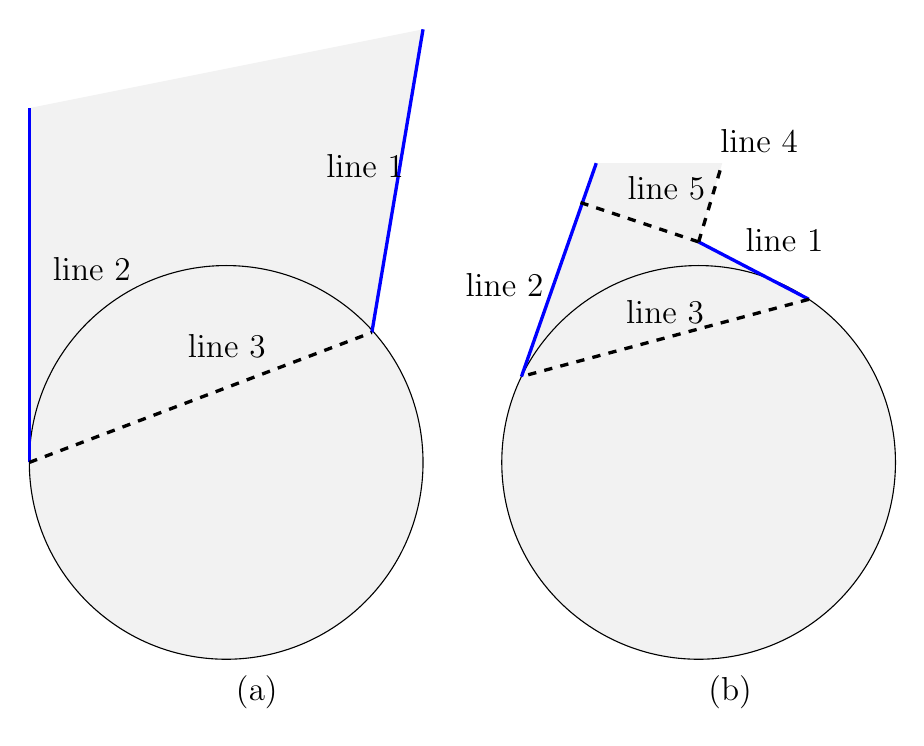
\begin{tikzpicture}
% \fill[black!5] (-2.5,4.5) -- (-2.5,0) -- (1.85,1.65) -- (2.5,5.5) -- cycle;
% \draw[fill=black!5] (0,0) circle (2.5);

% \draw[blue,very thick] (1.85,1.65) -- (2.5,5.5);
% \draw[blue,very thick] (-2.5,0) -- (-2.5,4.5);
% \draw[blue,very thick] (-2.5,0) -- (1.85,1.65);

% \node[anchor=west, xshift=-70pt, yshift=-5pt] at (1.85,1.65) {\large line 3};
% \node[anchor=west, xshift=-20pt, yshift=60pt] at (1.85,1.65) {\large line 1};
% \node[anchor=west, xshift=5pt, yshift=70pt] at (-2.5,0) {\large line 2};

\fill[black!5] (-8.5,4.5) -- (-8.5,0) -- (-4.15,1.65) -- (-3.5,5.5) -- cycle;
\draw[fill=black!5] (-6,0) circle (2.5);

\draw[blue,very thick] (-4.15,1.65) -- (-3.5,5.5);
\draw[blue,very thick] (-8.5,0) -- (-8.5,4.5);
\draw[black,very thick, dashed] (-8.5,0) -- (-4.15,1.65);

\node[anchor=west, xshift=-70pt, yshift=-5pt] at (-4.15,1.65) {\large line 3};
\node[anchor=west, xshift=-20pt, yshift=60pt] at (-4.15,1.65) {\large line 1};
\node[anchor=west, xshift=5pt, yshift=70pt] at (-8.5,0) {\large line 2};

\node[anchor=west, xshift=0pt, yshift=-83pt] at (-6,0) {\large (a)};

\fill[black!5] (-1.3,3.8) -- (-2.25,1.09) -- (1.4,2.0712) -- (0,2.8) -- (0.3,3.8) -- cycle;
\draw[fill=black!5] (0,0) circle (2.5);

% \draw[blue,very thick] (1.4,2.0712) -- (0,3);
% \draw[blue,very thick] (-2.45,0.5) -- (-1.6,4.8);
\draw[blue,very thick] (1.4,2.0712) -- (0,2.8);
\draw[blue,very thick] (-2.25,1.09) -- (-1.3,3.8);
\draw[black,very thick, dashed] (1.4,2.0712) -- (-2.25,1.09);

\draw[black,very thick, dashed] (0,2.8) -- (0.3,3.8);
\draw[black,very thick, dashed] (0,2.8) -- (-1.5,3.3);


\node[anchor=west, xshift=40pt, yshift=40pt] at (-2.45,0.5) {\large line 3};
\node[anchor=west, xshift=-15pt, yshift=15pt] at (1,2.3) {\large line 1};
\node[anchor=west, xshift=-18pt, yshift=50pt] at (-2.45,0.5) {\large line 2};
\node[anchor=west, xshift=10pt, yshift=-12pt] at (-0.2,4.5) {\large line 4};
\node[anchor=west, xshift=-15pt, yshift=8pt] at (-0.5,3.2) {\large line 5};

\node[anchor=west, xshift=0pt, yshift=-83pt] at (0,0) {\large (b)};


\end{tikzpicture}